\documentclass[12pt]{article}

% LuaLaTeX: fontspec + polyglossia для корректной работы с кириллицей
\usepackage{fontspec}
\defaultfontfeatures{Ligatures=TeX,Scale=MatchLowercase}
\setmainfont{Alice-Regular}[Path=font/,Extension=.ttf]
\newfontfamily\cyrillicfont{Alice-Regular}[Path=font/,Extension=.ttf]
\usepackage{polyglossia}
\setmainlanguage{russian}

\usepackage[style=numeric, backend=biber]{biblatex} % Обязательный пакет для корректной сборки
\addbibresource{references.bib}
\usepackage{graphicx}        						% Графика
\usepackage[protrusion=false]{microtype}       						% Микротипографика
\newfontfamily\cyrillicfonttt{Alice-Regular}[Path=font/,Extension=.ttf]
\usepackage{amssymb}        						% Математические символы
\usepackage{amsmath}        						% Математика
\usepackage{longtable}       						% Таблицы с разрывом страниц
\usepackage{tikz}           						% Рисование
\usepackage{circuitikz}     						% Электрические схемы
\usepackage{fix-cm}         						% Чтобы работал большой размер шрифта
\usepackage{anyfontsize}    						% Для любого размера шрифта
\usepackage{listings}       						% Для отображения кода
\usepackage{xcolor}         						% Для работы с цветами
% Настройка отображения кода (listings)
\lstdefinelanguage{MATLAB}{
	morekeywords={function,end,if,else,for,while,plot,mesh,surf,hold,on,legend},
	sensitive=true,
	morecomment=[l]{\%}
}
\lstset{
	language=MATLAB,
	basicstyle=\ttfamily\small,
	numbers=left,
	numberstyle=\tiny,
	stepnumber=1,
	numbersep=6pt,
	backgroundcolor=\color{gray!8},
	frame=single,
	rulecolor=\color{gray!40},
	breaklines=true,
	postbreak=\raisebox{0ex}[0ex][0ex]{\ensuremath{\hookrightarrow\ }},
	showstringspaces=false
}
\usepackage{fancyhdr}        						% Колонтитулы
\usepackage[a4paper,left=20mm,right=20mm,top=20mm,bottom=20mm]{geometry}

\title{
	МИНОБРНАУКИ РОССИИ

	федеральное государственное автономное образовательное учреждение

	высшего образования

	«Национальный исследовательский университет
	«Московский институт электронной техники»
	\vspace{2em}
}
\author{
	Андреев И. А.
}
\date{}

\begin{document}

\maketitle
\thispagestyle{fancy}

\begin{center}
\Large Лабораторная работа №1\\
по дисциплине «Квантовая механика»
\end{center}

\begin{center}
\Large Вариант 1
\end{center}

\vspace{12em}

\begin{table}[h]
\noindent
\begin{tabular*}{\textwidth}{@{\extracolsep{\fill}} p{0.48\textwidth} p{0.52\textwidth}}
Студент, группа & Андреев Иван Алексеевич, ЭН-$25$ \\
[0.5em] Руководитель & Журавлёв Максим Николаевич
\end{tabular*}
\end{table}

\fancyhf{}
\cfoot{Москва 2026}

\pagebreak

\section{Задание 1. Построение и оформление 2D-графиков волновых функций}

\subsection{Построить на одном графике $\psi_1(x)$ и $\psi_2(x)$ в атомных единицах}

\subsection{Отобразить потенциальную энергию $V_1(x)$ на том же графике пунктирной линией}

\begin{figure}[h]
\centering
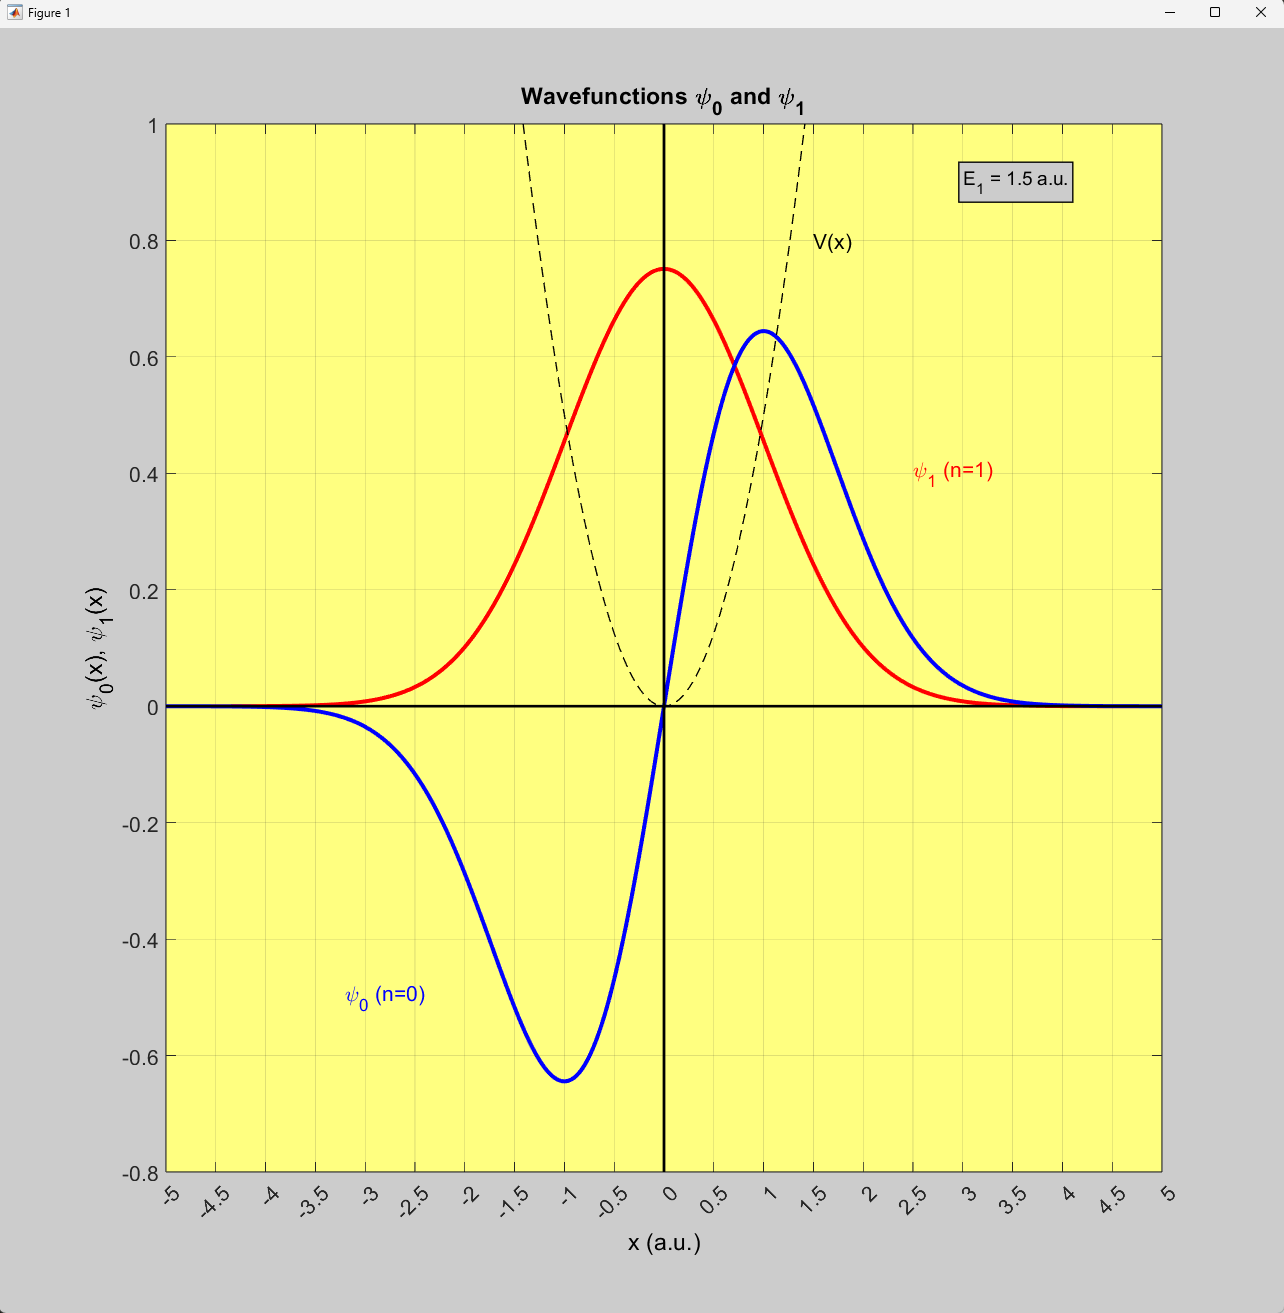
\includegraphics[width=\textwidth]{Task1.png}
\caption{Волновые функции $\psi_1(x)$ и $\psi_2(x)$}
\label{fig:task1}
\end{figure}

\subsection{Оформить график в соответствии в требованиями ниже :}

\begin{itemize}
\item Волновые функции $\psi_1(x)$ и $\psi_2(x)$ должны быть представлены разными цветами.
\item Изменить цвет фона и рабочей области.
\item Изменить цвет и размер названий осей и заголовка графика.
\item Оформить метки на координатных осях.
\item Изменить число меток на координатных осях и число линий сетки в рабочей области.
\item Выводить подписи уровней $\psi_1(x)$ и $\psi_2(x)$, указывать что координаты в атомных единицах.
\item Добавить текстовый вывод собственной энергии для одного состояния $E_1 = 1.5\text{ a.u.}$
\end{itemize}

Выполнение задач 1.1-1.2 явно видно на изображении \ref{fig:task1}. 
Выполнение требований к оформлению помечено в исходном коде в файле \textbf{Task1.m}, лежащем внутри архива 
с отчётом, с указанием пунктов.

\section{Задание 2. Построение и оформление 3D-графиков орбиталей атома водорода}

\subsection{Выбрать орбиталь \textbf{1s}}

\subsection{Построить поверхность, используя последовательно функции $\textbf{plot3}\to\textbf{mesh}\to\textbf{surf}$}

\subsection{Продемонстрировать различные цветовые карты: \textbf{jet}, \textbf{hot}, \textbf{bone}}

\begin{figure}[h]
\centering
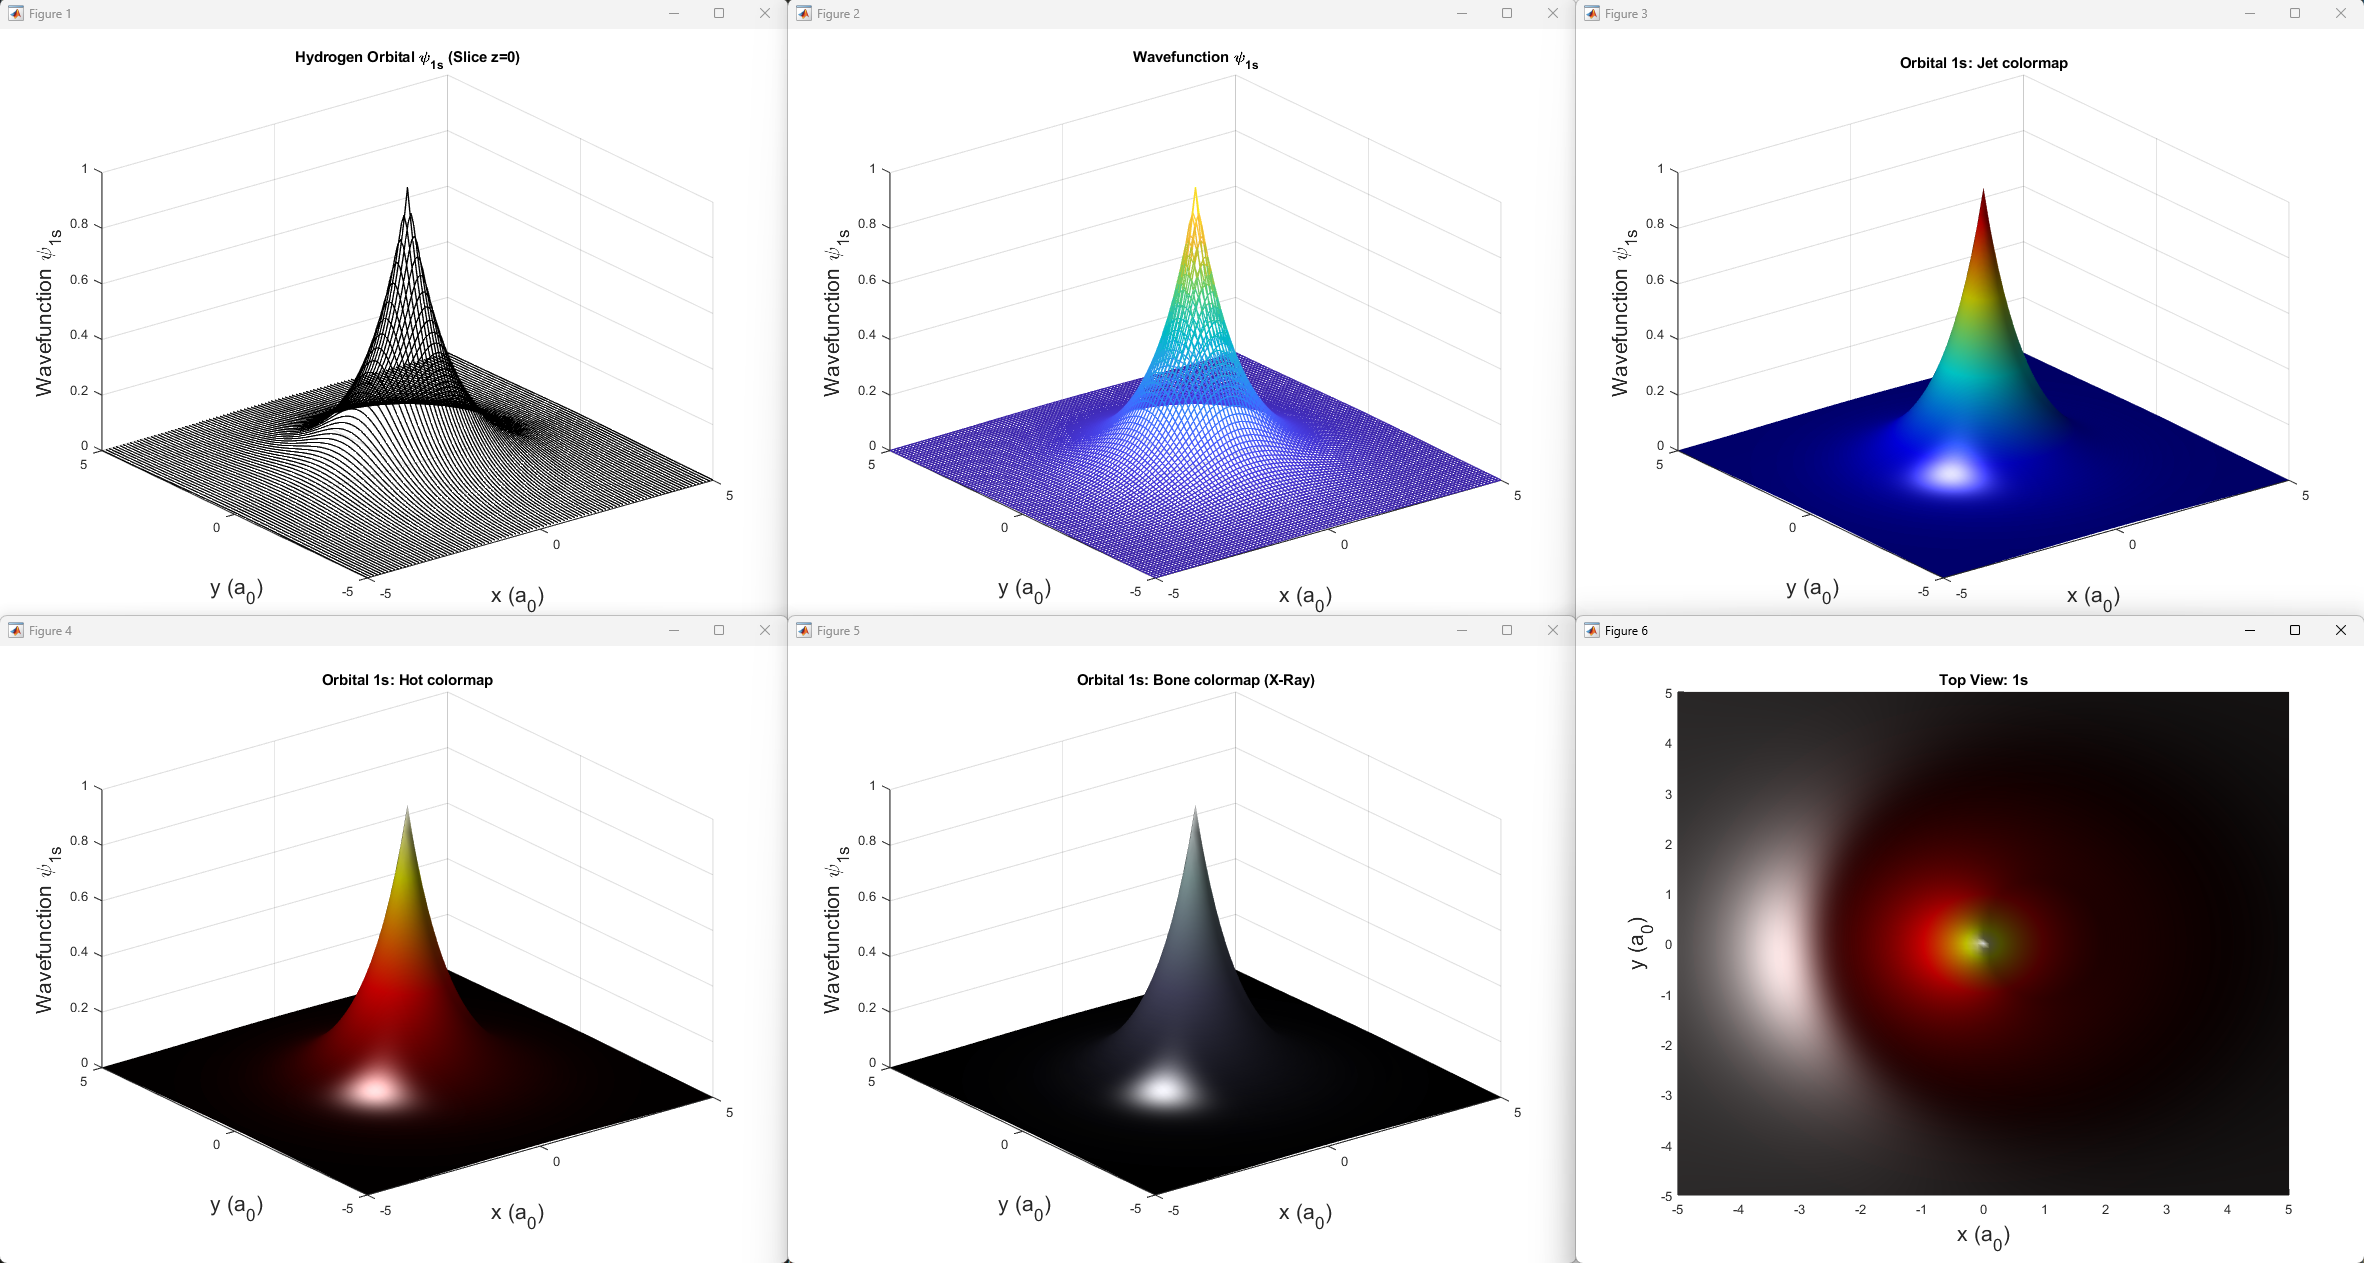
\includegraphics[width=\textwidth]{Task2.png}
\caption{Орбиталь \textbf{1s}}
\label{fig:task2}
\end{figure}

\subsection{Оформить график в соответствии с требованиями ниже :}

\begin{itemize}
\item В режимах \textbf{plot3} и \textbf{mesh} настроить цвет и толщину линий.
\item Продемонстрировать команду \textbf{shading interp}.
\item Добавить освещение сцены с помощью команд \textbf{lighting phong} и \textbf{camlight}.
\item Подобрать и применить цветовую карту: \textbf{jet} или \textbf{hot}.
\item Подписать оси, добавить заголовок, изменить размер шрифта меток.
\item Продемонстрировать \textbf{2D}-проекцию орбитали.
\end{itemize}

Выполнение задач 2.1-2.3 явно видно на изображении \ref{fig:task2}. 
Выполнение требований к оформлению помечено в исходном коде в файле \textbf{Task2.m}, лежащем внутри архива 
с отчётом, с указанием пунктов.

\section{Контрольные вопросы}

\subsection{Посмотрите в окно Workspace после выполнения скрипта с 3D-графиком. 
Чем отличаются размеры переменных $x$ и $X$, полученных после команды meshgrid?}

Переменная $x$ имеет размерность $1\text{x}101 \text{ double}$, а переменная $X$ имеет 
размерность $101\text{x}101 \text{ double}$.

\subsection{Запустите примеры. Чем визуально отличается результат работы команды \textbf{plot3} от команды \textbf{surf}?}

Команда \textbf{plot3} строит трёхмерный график в виде линий, а команда \textbf{surf} строит трёхмерный график в виде поверхности.

\subsection{В файле HarmonicOscillator.m используется команда hold on. 
Что произойдет с графиком потенциала, если эту команду удалить и запустить скрипт снова?}

Если удалить команду hold on, то график потенциала будет перерисован поверх графиков 
волновых функций, что сделает их невидимыми.

\subsection{При построении орбитали командой surf(X, Y, Z), что именно откладывается 
по вертикальной оси Z? Почему график может уходить «вниз» (в отрицательную область)?}

По вертикальной оси Z откладывается значение функции $\psi_{1s}(x,y)$, которая может 
принимать как положительные, так и отрицательные значения. График может уходить 
«вниз» (в отрицательную область), потому что функция $\psi_{1s}(x,y)$ может принимать 
отрицательные значения в некоторых областях пространства, например в тех случаях, когда 
волновая функция пропорциональна $x$ или $xy$, которые могут принимать отрицательные значения.

\subsection{Найдите в коде строчку, где задается шаг сетки. 
Что изменится в виде поверхности, если уменьшить это число в 2 раза?}

Шаг сетки задается в строке, где определяется диапазон значений для переменных 
$x$ и $y$. Если уменьшить этот шаг в 2 раза, то поверхность будет построена с 
большей детализацией, так как будет использоваться больше точек для построения 
графика. Это может сделать график более гладким и точным, но также может увеличить 
время выполнения скрипта.

\subsection{В файле HarmonicOscillator.m функция plot возвращает массив дескрипторов 
hPl. Как с помощью индексации изменить свойства только одной из нескольких линий, 
построенных одной командой?}

Можно использовать следующий код :

\begin{figure}[h]
\centering
\includegraphics[width=\textwidth]{Matlab1.png}
\caption{Изменение свойств одной из линий, построенных одной командой}
\label{fig:matlab1}
\end{figure}

\end{document}